% Profit Optimization ROI Attribution (Waterfall Chart)
% Replaces: tab:profit-optimization-ablation in section_profit_optimization_results.tex
% Shows how each component contributes to the 7.9% total ROI improvement

\begin{figure}[htbp]
\centering
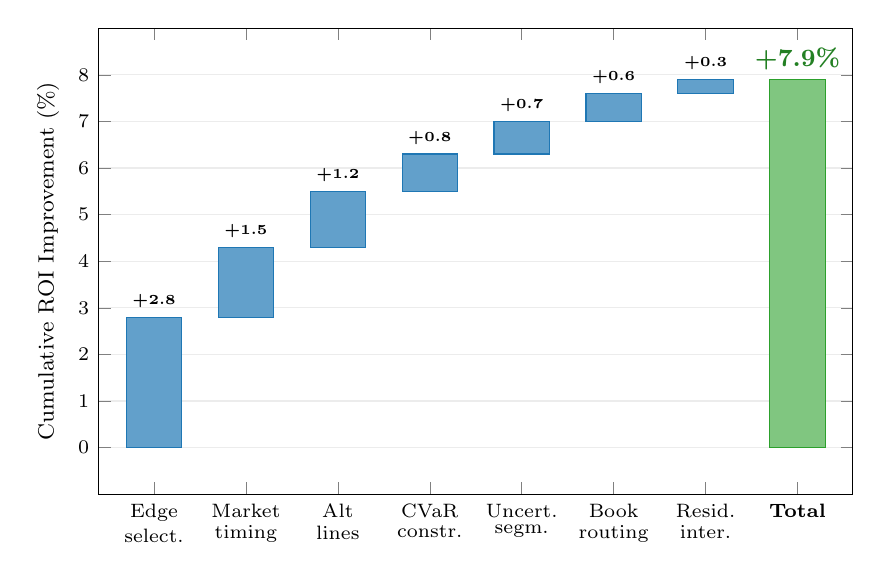
\begin{tikzpicture}
\definecolor{accent}{RGB}{31,119,180}
\definecolor{accentGreen}{RGB}{44,160,44}
\definecolor{accentRed}{RGB}{214,39,40}

% Waterfall chart via stacking
\begin{axis}[
  width=0.92\textwidth,
  height=7.5cm,
  ybar stacked,
  bar width=20pt,
  ylabel={Cumulative ROI Improvement (\%)},
  ylabel style={font=\footnotesize},
  ymin=-1, ymax=9,
  xtick={1,2,3,4,5,6,7,8},
  xticklabels={
    {\shortstack{Edge\\select.}},
    {\shortstack{Market\\timing}},
    {\shortstack{Alt\\lines}},
    {\shortstack{CVaR\\constr.}},
    {\shortstack{Uncert.\\segm.}},
    {\shortstack{Book\\routing}},
    {\shortstack{Resid.\\inter.}},
    {\textbf{Total}}
  },
  xticklabel style={font=\scriptsize},
  ytick={0,1,2,3,4,5,6,7,8},
  yticklabel style={font=\scriptsize},
  grid=major,
  grid style={gray!15},
  xmajorgrids=false,
  enlarge x limits={abs=0.6},
]

% Invisible base (lifts the visible bars to correct cumulative position)
\addplot[fill=none, draw=none, forget plot] coordinates {
  (1, 0) (2, 2.8) (3, 4.3) (4, 5.5) (5, 6.3) (6, 7.0) (7, 7.6) (8, 0)
};

% Visible incremental bars
\addplot[fill=accent!70, draw=accent] coordinates {
  (1, 2.8) (2, 1.5) (3, 1.2) (4, 0.8) (5, 0.7) (6, 0.6) (7, 0.3) (8, 0)
};

% Total bar (different color, from 0)
\addplot[fill=accentGreen!60, draw=accentGreen, forget plot] coordinates {
  (1, 0) (2, 0) (3, 0) (4, 0) (5, 0) (6, 0) (7, 0) (8, 7.9)
};

% Value labels on bars
\node[font=\tiny\bfseries, anchor=south] at (axis cs:1,2.8) {+2.8};
\node[font=\tiny\bfseries, anchor=south] at (axis cs:2,4.3) {+1.5};
\node[font=\tiny\bfseries, anchor=south] at (axis cs:3,5.5) {+1.2};
\node[font=\tiny\bfseries, anchor=south] at (axis cs:4,6.3) {+0.8};
\node[font=\tiny\bfseries, anchor=south] at (axis cs:5,7.0) {+0.7};
\node[font=\tiny\bfseries, anchor=south] at (axis cs:6,7.6) {+0.6};
\node[font=\tiny\bfseries, anchor=south] at (axis cs:7,7.9) {+0.3};
\node[font=\small\bfseries, text=accentGreen!80!black, anchor=south] at (axis cs:8,7.9) {+7.9\%};

% Starting/ending annotations
\node[font=\tiny, text=accentRed, anchor=east, align=right] at (axis cs:0.5,-0.5)
  {Before: $-$6.2\% ROI};
\node[font=\tiny, text=accentGreen!80!black, anchor=west, align=left] at (axis cs:8.5,7.9)
  {After: +1.7\% ROI};

\end{axis}
\end{tikzpicture}
\caption[Profit optimization ROI attribution]{ROI attribution by optimization component (waterfall chart). Edge-based selection contributes the largest single improvement (+2.8\%), followed by market timing (+1.5\%) and alternative line analysis (+1.2\%). The complete optimization framework transforms $-6.2\%$ baseline ROI to $+1.7\%$ net ROI, a total swing of +7.9 percentage points.}
\label{fig:profit-attribution-chart}
\end{figure}
